\documentclass{beamer}

\usepackage{iansslides}

\begin{document}

\section{Graphs}

\begin{frame}{Seven Bridges of K{\"o}nigsberg}
    \begin{alertblock}{Is it possible to walk through the city crossing each of the seven bridges exactly once?}
    \begin{center}
      %\includegraphics[width=9cm]{img/konigsberg.png}
    \end{center}
  \end{alertblock}
    \citeurl{www.nature.com/nbt/journal/v29/n11}
  \end{frame}
  
  \begin{frame}{Leonhard Euler}  
    \begin{columns}[T]
      \begin{column}{0.3\textwidth}
        %\includegraphics[height=2in]{img/euler.jpg}
      \end{column}
      \begin{column}{0.65\textwidth}
        \begin{itemize}
          \setlength\itemsep{3mm}
          \item Born 1707 in Basel, Switzerland.
          \item Euler's identity: $\mathrm{e}^{i \pi} + 1 = 0$.
          \item Solved the Bridges of K{\"o}nigsberg.
          \item It's not possible.
        \end{itemize}
      \end{column}
    
    \end{columns}
  \end{frame}
  
  \begin{frame}{K{\"o}nigsberg (multi)graph}
    \vspace{10mm}
    \begin{adjustbox}{max width={0.9\textwidth},center} 
      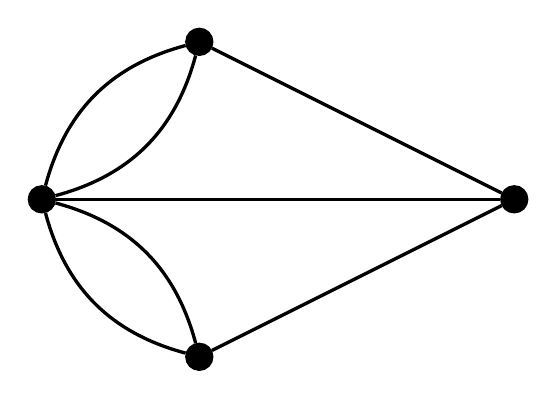
\begin{tikzpicture}
        \begin{scope}[every node/.style={circle,thick,draw=black,fill=black}]
          \node[] (A) at (0,0) {};
          \node[] (B) at (2,2) {};
          \node[] (C) at (6,0) {};
          \node[] (D) at (2,-2) {};
        \end{scope}
        \begin{scope}[every edge/.style={draw=black,very thick}]
          \path (A) edge[bend right=30] (B);
          \path (A) edge[bend left=30] (B);
          \path (A) edge[bend right=30] (D);
          \path (A) edge[bend left=30]  (D);
          \path (B) edge (C);
          \path (A) edge (C);
          \path (D) edge (C);
        \end{scope}
      \end{tikzpicture}
    \end{adjustbox}
  \end{frame}
  
  \begin{frame}{Graphs}
    \begin{alertblock}{Definition}
    A \emph{graph} consists of a finite set $V$ and a set $E$ of 2-subsets of $V$.
    \end{alertblock}
    \vspace{4mm}
    \begin{description}
      \setlength\itemsep{3mm}
      \item[$2$-subset] -- a subset with two elements.
      \item[Vertices] -- the elements of the set $V$ are called vertices.
      \item[Edges] -- the elements of $E$ are called edges.
      \item[$G = (V,E)$] -- this is the way we write the graph $G$ consists of the vertex set $V$ and the edge set $E$.
    \end{description}
  \end{frame}
  
  
  \begin{frame}{Drawings of graphs}
    \begin{adjustbox}{max width={0.9\textwidth}, center}
      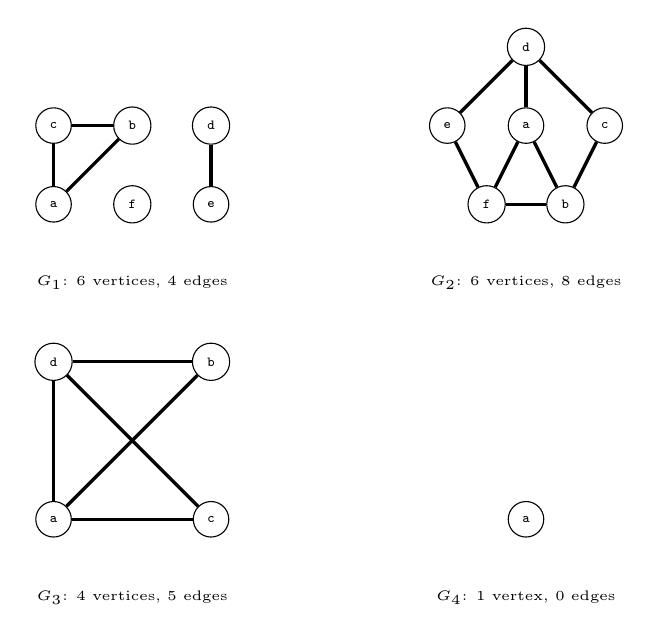
\begin{tikzpicture}
        \begin{scope}
          \begin{scope}[every node/.style={draw=black, circle}]
            \node (a) at (0,0) {\tiny \texttt{a}};
            \node (b) at (2,2) {\tiny \texttt{b}};
            \node (c) at (2,0) {\tiny \texttt{c}};
            \node (d) at (0,2) {\tiny \texttt{d}};
          \end{scope}
          \begin{scope}[every edge/.style={draw=black, very thick}]
            \path (a) edge (b);
            \path (a) edge (c);
            \path (a) edge (d);
            \path (d) edge (b);
            \path (d) edge (c);
          \end{scope}
          \node at (1,-1) {\tiny $G_3$: 4 vertices, 5 edges};
        \end{scope}
        \begin{scope}[yshift=4cm]
          \begin{scope}[every node/.style={draw=black, circle}]
            \node (a) at (0,0) {\tiny \texttt{a}};
            \node (b) at (1,1) {\tiny \texttt{b}};
            \node (c) at (0,1) {\tiny \texttt{c}};
            \node (d) at (2,1) {\tiny \texttt{d}};
            \node (e) at (2,0) {\tiny \texttt{e}};
            \node (f) at (1,0) {\tiny \texttt{f}};
          \end{scope}
          \begin{scope}[every edge/.style={draw=black, very thick}]
            \path (a) edge (b);
            \path (a) edge (c);
            \path (b) edge (c);
            \path (d) edge (e);
          \end{scope}
          \node at (1,-1) {\tiny $G_1$: 6 vertices, 4 edges};
        \end{scope}
        \begin{scope}[xshift=6cm,yshift=4cm]
          \begin{scope}[every node/.style={draw=black, circle}]
            \node (a) at ( 0  ,1) {\tiny \texttt{a}};
            \node (b) at ( 0.5,0) {\tiny \texttt{b}};
            \node (c) at ( 1  ,1) {\tiny \texttt{c}};
            \node (d) at ( 0  ,2) {\tiny \texttt{d}};
            \node (e) at (-1  ,1) {\tiny \texttt{e}};
            \node (f) at (-0.5,0) {\tiny \texttt{f}};
          \end{scope}
          \begin{scope}[every edge/.style={draw=black, very thick}]
            \path (a) edge (b);
            \path (a) edge (d);
            \path (a) edge (f);
            \path (b) edge (c);
            \path (c) edge (d);
            \path (d) edge (e);
            \path (e) edge (f);
            \path (f) edge (b);
          \end{scope}
          \node at (0,-1) {\tiny $G_2$: 6 vertices, 8 edges};
        \end{scope}
        \begin{scope}[xshift=6cm]
          \begin{scope}[every node/.style={draw=black, circle}]
            \node (a) at (0,0) {\tiny \texttt{a}};
          \end{scope}
          \node at (0,-1) {\tiny $G_4$: 1 vertex, 0 edges};
        \end{scope}
      \end{tikzpicture}
    \end{adjustbox}
  \end{frame}
  
  \begin{frame}{Drawings are not definitions}
    \vspace{8mm}
    \begin{adjustbox}{width={0.3\textwidth}, center}
      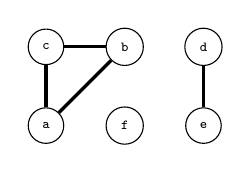
\begin{tikzpicture}
        \begin{scope}
          \begin{scope}[every node/.style={draw=black, circle}]
            \node (a) at (0,0) {\tiny \texttt{a}};
            \node (b) at (1,1) {\tiny \texttt{b}};
            \node (c) at (0,1) {\tiny \texttt{c}};
            \node (d) at (2,1) {\tiny \texttt{d}};
            \node (e) at (2,0) {\tiny \texttt{e}};
            \node (f) at (1,0) {\tiny \texttt{f}};
          \end{scope}
          \begin{scope}[every edge/.style={draw=black, very thick}]
            \path (a) edge (b);
            \path (a) edge (c);
            \path (b) edge (c);
            \path (d) edge (e);
          \end{scope}
        \end{scope}
      \end{tikzpicture}
    \end{adjustbox}
    \vspace{4mm}
    \begin{description}
      \setlength\itemsep{4mm}
      \item[$V$] $= \{a,b,c,d,e,f\}$
      \item[$E$] $= \{\{a,b\},\{a,c\},\{b,c\},\{d,e\}\}$
    \end{description}
  \end{frame}
  
  
  \begin{frame}{A better example}
    \begin{adjustbox}{max width={0.9\textwidth},center} 
      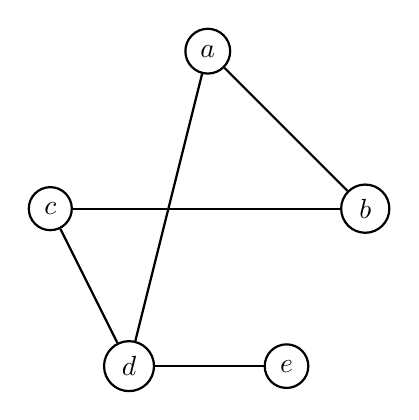
\begin{tikzpicture}
        \begin{scope}[every node/.style={circle,thick,draw}]
          \node (a) at (2,4) {$a$};
          \node (b) at (4,2) {$b$};
          \node (e) at (3,0) {$e$};
          \node (d) at (1,0) {$d$};
          \node (c) at (0,2) {$c$};
        \end{scope}
        \begin{scope}[every edge/.style={draw=black,thick}]
          \path (a) edge (b);
          \path (a) edge (d);
          \path (b) edge (c);
          \path (e) edge (d);
          \path (d) edge (c);
        \end{scope}
      \end{tikzpicture}
    \end{adjustbox}
    \vspace{0.1cm}
    \begin{block}{Exercise}
    Determine the vertex set, edge set and adjacency list of this graph.
    \end{block}
    
    \citeurl{global.oup.com/booksites/content/9780198507185/}
  \end{frame}
  
  \begin{frame}{Adjanceny list}
    \begin{center}
      \begin{tabular}{c@{\hskip 1cm}c@{\hskip 1cm}c@{\hskip 1cm}c@{\hskip 1cm}c}
        $a$ & $b$ & $c$ & $d$ & $e$ \\
        \midrule
        $b$ & $a$ & $b$ & $a$ & $d$ \\
        $d$ & $c$ & $d$ & $c$ &     \\
            &     &     & $e$ &     \\
      \end{tabular}
    \end{center}
    Useful (sometimes) for representing graphs in code.
  \end{frame}
  
  
  \begin{frame}{Another better example}
    \begin{adjustbox}{max width={0.9\textwidth},center} 
      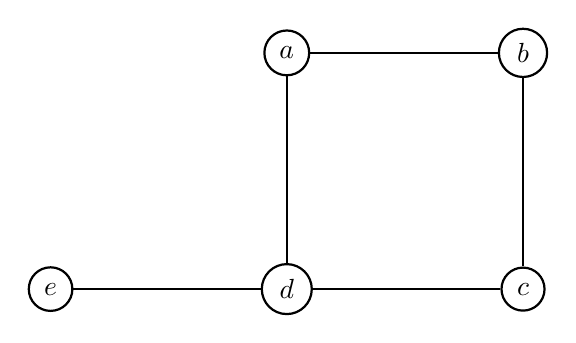
\begin{tikzpicture}
        \begin{scope}[every node/.style={circle,thick,draw}]
          \node (a) at (0,3) {$a$};
          \node (b) at (3,3) {$b$};
          \node (e) at (-3,0) {$e$};
          \node (d) at (0,0) {$d$};
          \node (c) at (3,0) {$c$};
        \end{scope}
        \begin{scope}[every edge/.style={draw=black,thick}]
          \path (a) edge (b);
          \path (a) edge (d);
          \path (b) edge (c);
          \path (e) edge (d);
          \path (d) edge (c);
        \end{scope}
      \end{tikzpicture}
    \end{adjustbox}
    \vspace{0.1cm}
    \begin{block}{Exercise}
    Determine the vertex set, edge set and adjacency list of this graph.
    \end{block}
    
    \citeurl{global.oup.com/booksites/content/9780198507185/}
  \end{frame}
  
  \begin{frame}{Complete graph $K_n$}
    \begin{adjustbox}{max width={0.9\textwidth},center} 
      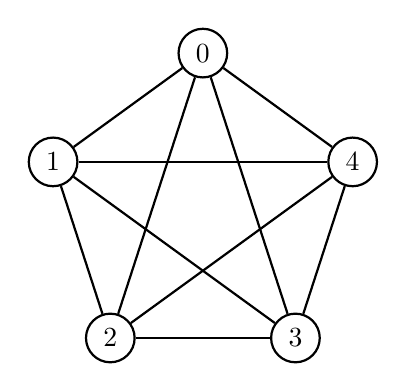
\begin{tikzpicture}
        \begin{scope}[every node/.style={circle,thick,draw}]
        \foreach \s in {0,...,4}
        {
          \node (\s) at ({72 * \s + 90}:2) {$\s$};
        }
        \end{scope}
        \begin{scope}[every edge/.style={draw=black,thick}]
          \path (0) edge (1);
          \path (0) edge (2);
          \path (0) edge (3);
          \path (0) edge (4);
          \path (1) edge (2);
          \path (1) edge (3);
          \path (1) edge (4);
          \path (2) edge (3);
          \path (2) edge (4);
          \path (3) edge (4);
        \end{scope}
      \end{tikzpicture}
    \end{adjustbox}
    \vspace{0.1cm}
    \begin{block}{Exercise}
    Determine the vertex set, edge set and adjacency list of $K_5$.
    \end{block}
  \end{frame}
  
  
  \begin{frame}{Wheel graph $W_n$}
    \begin{adjustbox}{max width={0.9\textwidth},center} 
      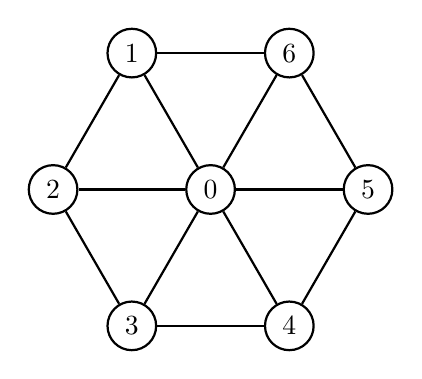
\begin{tikzpicture}
        \begin{scope}[every node/.style={circle,thick,draw}]
          \foreach \s in {1,...,6}
          {
            \node (\s) at ({60 * \s + 60}:2) {$\s$};
          }
          \node (0) at (0:0) {$0$};
        \end{scope}
        \begin{scope}[every edge/.style={draw=black,thick}]
          \path (0) edge (1);
          \path (0) edge (2);
          \path (0) edge (3);
          \path (0) edge (4);
          \path (0) edge (5);
          \path (0) edge (6);
          \path (1) edge (2);
          \path (2) edge (3);
          \path (3) edge (4);
          \path (4) edge (5);
          \path (5) edge (6);
          \path (6) edge (1);
        \end{scope}
      \end{tikzpicture}
    \end{adjustbox}
    \vspace{0.1cm}
    \begin{block}{Exercise}
    Determine the vertex set, edge set and adjacency list of $W_6$.
    \end{block}
  \end{frame}
  
  
  \begin{frame}{Degree of a vertex}
  
    \begin{definition}
      The degree of a vertex is the number of edges that contain it.
    \end{definition}
      
    \begin{center}
      \begin{columns}
        \begin{column}{0.2\textwidth}
          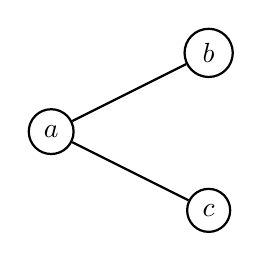
\begin{tikzpicture}
            \begin{scope}[every node/.style={circle,thick,draw}]
              \node (a) at (0,0) {$a$};
              \node (b) at (2,1) {$b$};
              \node (c) at (2,-1) {$c$};
            \end{scope}
            \begin{scope}[every edge/.style={draw=black,thick}]
              \path (a) edge (b);
              \path (a) edge (c);
            \end{scope}
          \end{tikzpicture}
        \end{column}
        \begin{column}{0.5\textwidth}
            The degree of the vertex $a$ is 2.
        \end{column}
      \end{columns}
    \end{center}
  
    \begin{block}{Exercise}
      For each of the vertices on the previous slide, determine its degree.
    \end{block}
  
  \end{frame}
  
  
  
  \begin{frame}{Sum of degrees}
    \vspace{-4mm}
    \begin{theorem}
      The sum of the degrees of the vertices of a graph $G = (V,E)$ is equal to twice the number of edges:
        \[ \sum_{\mathrm{v} \in V} \delta (\mathrm{v}) = 2 | E | \]
    \end{theorem}
    \vspace{-4mm}
    \begin{columns}[T]
      \begin{column}{0.75\textwidth}
        \begin{proof}
          The degree $\delta (\mathrm{v})$ of a vertex $\mathrm{v}$ is equal to the number of edges incident on it.
          Every edge is incident on two vertices.
          So every edge contributes $1$ to the degrees of two distinct vertices.
          Therefore every edge contributes $2$ to the sum total of the degrees of all the vertices.
        \end{proof}
      \end{column}
      \begin{column}{0.2\textwidth}
        \begin{center}
          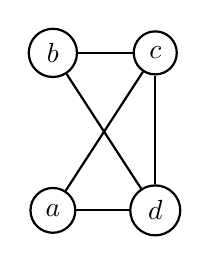
\begin{tikzpicture}
            \begin{scope}[every node/.style={circle,thick,draw}]
              \node (a) at (0,0) {$a$};
              \node (b) at (0,2) {$b$};
              \node (c) at (1.3,2) {$c$};
              \node (d) at (1.3,0) {$d$};
            \end{scope}
            \begin{scope}[every edge/.style={draw=black,thick}]
              \path (b) edge (c);
              \path (b) edge (d);
              \path (d) edge (c);
              \path (c) edge (a);
              \path (d) edge (a);
            \end{scope}
          \end{tikzpicture}
        \end{center}
      \end{column}
    \end{columns}
  \end{frame}
  
  \begin{frame}{Even and odd vertices}
    \vspace{-4mm}
    \begin{definition}
      A vertex is an odd vertex if its degree is odd, and it is an even vertex if its degree is even.
      The set of all odd vertices is denoted $V_o$ and the set of all even vertices is denoted $V_e$.
    \end{definition}
    \begin{center}
      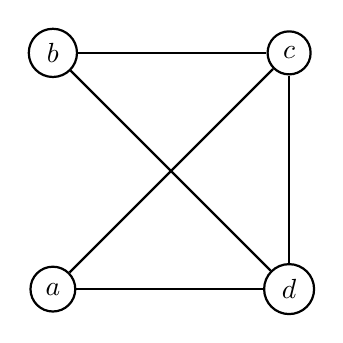
\begin{tikzpicture}
        \begin{scope}[every node/.style={circle,thick,draw}]
          \node (a) at (0,0) {$a$};
          \node (b) at (0,3) {$b$};
          \node (c) at (3,3) {$c$};
          \node (d) at (3,0) {$d$};
        \end{scope}
        \begin{scope}[every edge/.style={draw=black,thick}]
          \path (b) edge (c);
          \path (b) edge (d);
          \path (d) edge (c);
          \path (c) edge (a);
          \path (d) edge (a);
        \end{scope}
      \end{tikzpicture}
    \end{center}
    \begin{block}{Exercise}
      Which of the above vertices are even, and which are odd?
    \end{block}
  \end{frame}
  
  \begin{frame}{Handshaking lemma}
  
    \begin{lemma}
      The number of odd vertices $| V_o |$ in a graph is even.
    \end{lemma}
  
    \begin{proof}
      The sets $V_o$ and $V_e$ are disjoint (i.e.\ they don't have any elements in common.)
      Also, every vertex is either in $V_o$ or $V_e$.
      Therefore $V = V_o \cup V_e$ and $|V| = |V_o| + |V_e|$.
      
      Furthermore:
        \[ \sum_{\mathrm{v} \in V_o} \delta(\mathrm{v}) + \sum_{\mathrm{v} \in V_e} \delta(\mathrm{v}) = 2 |E| \]
  
      Both $2|E|$ and $\sum_{\mathrm{v} \in V_e} \delta(\mathrm{v})$ are even, so $\sum_{\mathrm{v} \in V_o} \delta(\mathrm{v})$ must be.
      Since $\delta(\mathrm{v})$ is odd for every $\mathrm{v}$ in $V_o$, this must mean that $|V_o|$ is even.
    \end{proof}
  
  \end{frame}
  
  
  \begin{frame}{Sets of K{\"o}nigsberg}
    \begin{adjustbox}{width={0.4\textwidth},center} 
      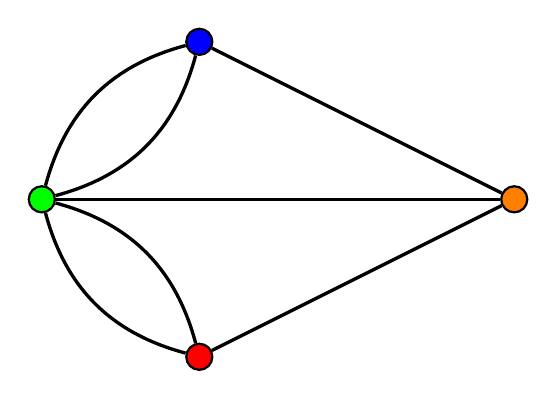
\begin{tikzpicture}
        \begin{scope}[every node/.style={circle,thick,draw=black,fill=black}]
          \node[fill=green]  (A) at (0,0) {};
          \node[fill=blue]   (B) at (2,2) {};
          \node[fill=orange] (C) at (6,0) {};
          \node[fill=red]    (D) at (2,-2) {};
        \end{scope}
        \begin{scope}[every edge/.style={draw=black,very thick}]
          \path (A) edge[bend right=30] (B);
          \path (A) edge[bend left=30] (B);
          \path (A) edge[bend right=30] (D);
          \path (A) edge[bend left=30]  (D);
          \path (B) edge (C);
          \path (A) edge (C);
          \path (D) edge (C);
        \end{scope}
      \end{tikzpicture}
    \end{adjustbox}
    \vspace{-2mm}
    $$V = \{G, B, O, R\}$$
    \vspace{-6mm}
    $$E = \{\{G, B\}, \{G, B\}, \{G, R\},\{G, R\}, \{B, O\}, \{G, O\},\{R, O\}\}$$
  
    \begin{alertblock}{Not a graph by our definition}
      Note that the Bridges of K{\"o}nigsberg graph above is not a graph, due to the repeated edges.
      It's a multi-graph.
    \end{alertblock}
  \end{frame}
  
  \begin{frame}{Defining different types of graphs}
    
    \begin{alertblock}{Our definition of a graph}
    The definition given above for a graph is not consistent with looped edges, directed edges or repeated edges. We only need to make small changes to the definition of a graph to allow for directed edges and repeated edges.
    \end{alertblock}
    
    \begin{description}
      \item[Repeated edges] start and end at the same vertices.
      \item[Directed edges] have a direction.
      \item[Looped edges] begin and end at the same vertex.
    \end{description}
    
    The application will determine the definition we want to use.
  \end{frame}
  
  
  
  \begin{frame}{Directed graph definition}
    \vspace{-4mm}
    \begin{definition}
    A \emph{directed graph} (digraph) consists of a finite set $V$ and a set $E$ of 2-tuples (ordered pairs of elements) from $V$.
    \end{definition}
    \vspace{0.2cm}
    \begin{description}
      \item[Looped edges] are allowed in this definition. A single one per vertex.
      \item[Multiple edges] between the same start and end vertices are not allowed. However, two edges are allowed between every pair of vertices so long as they have opposite directions.
      \item[Direct edges] use round brackets rather than curly braces: $E = \{ (a,b) \mid a,b \in V\}$.
    \end{description}
  \end{frame}
  
  
  \begin{frame}{Example directed graphs}
    \vspace{-6mm}
    \begin{columns}[T]
      \begin{column}{0.45\textwidth}
        \begin{center}
          \begin{adjustbox}{max width={0.9\textwidth}, center}
            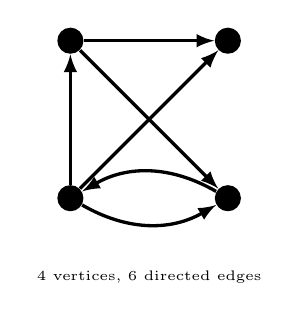
\begin{tikzpicture}
              \begin{scope}[every node/.style={fill=black, circle}]
                \node (a) at (0,0) {};
                \node (b) at (2,2) {};
                \node (c) at (2,0) {};
                \node (d) at (0,2) {};
              \end{scope}
              \begin{scope}[every edge/.style={draw=black, very thick, ->, >=latex}]
                \path (a) edge (b);
                \path (a) edge[bend right] (c);
                \path (c) edge[bend right] (a);
                \path (a) edge (d);
                \path (d) edge (b);
                \path (d) edge (c);
              \end{scope}
              \node at (1,-1) {\tiny 4 vertices, 6 directed edges};
            \end{tikzpicture}
          \end{adjustbox}
        \end{center}
      \end{column}
      \begin{column}{0.45\textwidth}
        \begin{center}
          \begin{adjustbox}{max width={0.9\textwidth}, center}
            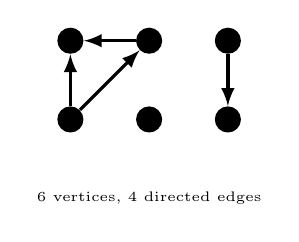
\begin{tikzpicture}
              \begin{scope}[every node/.style={fill=black, circle}]
                \node (a) at (0,0) {};
                \node (b) at (1,1) {};
                \node (c) at (0,1) {};
                \node (d) at (2,1) {};
                \node (e) at (2,0) {};
                \node (f) at (1,0) {};
              \end{scope}
              \begin{scope}[every edge/.style={draw=black, very thick, ->, >=latex}]
                \path (a) edge (b);
                \path (a) edge (c);
                \path (b) edge (c);
                \path (d) edge (e);
              \end{scope}
              \node at (1,-1) {\tiny 6 vertices, 4 directed edges};
            \end{tikzpicture}
          \end{adjustbox}
        \end{center}
      \end{column}
    \end{columns}
    \vspace{5mm}
    \begin{columns}
      \begin{column}{0.45\textwidth}
        \begin{center}
          \begin{adjustbox}{max width={0.9\textwidth}, center}
            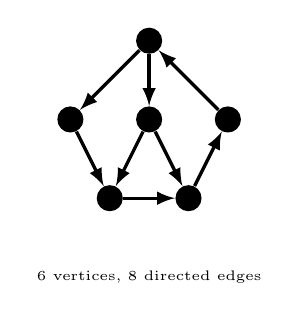
\begin{tikzpicture}
              \begin{scope}[every node/.style={fill=black, circle}]
                \node (a) at (1  ,1) {};
                \node (b) at (1.5,0) {};
                \node (c) at (2  ,1) {};
                \node (d) at (1  ,2) {};
                \node (e) at (0  ,1) {};
                \node (f) at (0.5,0) {};
              \end{scope}
              \begin{scope}[every edge/.style={draw=black, very thick, ->, >=latex}]
                \path (a) edge (b);
                \path (d) edge (a);
                \path (a) edge (f);
                \path (b) edge (c);
                \path (c) edge (d);
                \path (d) edge (e);
                \path (e) edge (f);
                \path (f) edge (b);
              \end{scope}
              \node at (1,-1) {\tiny 6 vertices, 8 directed edges};
            \end{tikzpicture}
          \end{adjustbox}
        \end{center}
      \end{column}
          \begin{column}{0.45\textwidth}
        \begin{center}
          \begin{adjustbox}{max width={0.9\textwidth}, center}
            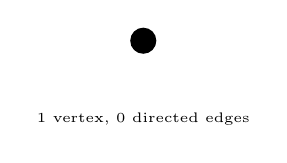
\begin{tikzpicture}
              \begin{scope}[every node/.style={fill=black, circle}]
                \node (a) at (0,0) {};
              \end{scope}
              \node at (0,-1) {\tiny 1 vertex, 0 directed edges};
            \end{tikzpicture}
          \end{adjustbox}
        \end{center}
      \end{column}
    \end{columns}
  \end{frame}
  
  
  
  \begin{frame}{Multigraph definition}
    \begin{definition}
    A \emph{multigraph} consists of a finite set $V$ and a multiset $E$ of 2-multisubsets from $V$.
    \end{definition}
    \vspace{0.2cm}
    \begin{description}
      \item[Multisets] are like sets, but the same element can be in the set more than once.
      \item[Directed multigraphs] are similar, but $E$ is a set of 2-tuples of elements in $V$.
    \end{description}
  \end{frame}
  
  \begin{frame}{Example multigraphs}
    \vspace{-10mm}
    \begin{columns}
      \begin{column}{0.45\textwidth}
        \begin{center}
          \begin{adjustbox}{max width={0.9\textwidth}, center}
            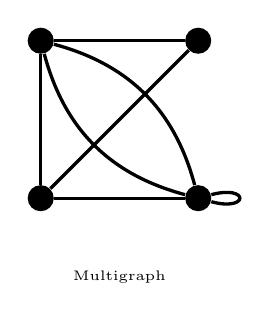
\begin{tikzpicture}[every loop/.style={}]
              \begin{scope}[every node/.style={fill=black, circle}]
                \node (a) at (0,0) {};
                \node (b) at (2,2) {};
                \node (c) at (2,0) {};
                \node (d) at (0,2) {};
              \end{scope}
              \begin{scope}[every edge/.style={draw=black, very thick}]
                \path (a) edge (b);
                \path (c) edge (a);
                \path (a) edge (d);
                \path (d) edge (b);
                \path (d) edge[bend right] (c);
                \path (d) edge[bend left] (c);
                \path (c) edge[loop right] (c);
              \end{scope}
              \node at (1,-1) {\tiny Multigraph};
            \end{tikzpicture}
          \end{adjustbox}
        \end{center}
      \end{column}
      \begin{column}{0.45\textwidth}
        \begin{center}
          \begin{adjustbox}{max width={0.9\textwidth}, center}
            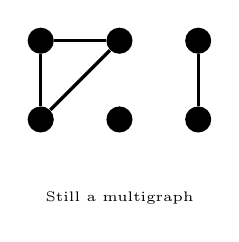
\begin{tikzpicture}
              \begin{scope}[every node/.style={fill=black, circle}]
                \node (a) at (0,0) {};
                \node (b) at (1,1) {};
                \node (c) at (0,1) {};
                \node (d) at (2,1) {};
                \node (e) at (2,0) {};
                \node (f) at (1,0) {};
              \end{scope}
              \begin{scope}[every edge/.style={draw=black, very thick}]
                \path (a) edge (b);
                \path (a) edge (c);
                \path (b) edge (c);
                \path (d) edge (e);
              \end{scope}
              \node at (1,-1) {\tiny Still a multigraph};
            \end{tikzpicture}
          \end{adjustbox}
        \end{center}
      \end{column}
    \end{columns}
    \vspace{5mm}
    \begin{columns}
      \begin{column}{0.45\textwidth}
        \begin{center}
          \begin{adjustbox}{max width={0.9\textwidth}, center}
            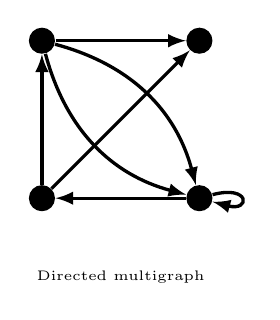
\begin{tikzpicture}[every loop/.style={}]
              \begin{scope}[every node/.style={fill=black, circle}]
                \node (a) at (0,0) {};
                \node (b) at (2,2) {};
                \node (c) at (2,0) {};
                \node (d) at (0,2) {};
              \end{scope}
              \begin{scope}[every edge/.style={draw=black, very thick, ->, >=latex}]
                \path (a) edge (b);
                \path (c) edge (a);
                \path (a) edge (d);
                \path (d) edge (b);
                \path (d) edge[bend right] (c);
                \path (d) edge[bend left] (c);
                \path (c) edge[loop right] (c);
              \end{scope}
              \node at (1,-1) {\tiny Directed multigraph};
            \end{tikzpicture}
          \end{adjustbox}
        \end{center}
      \end{column}
      \begin{column}{0.45\textwidth}
        \begin{center}
          \begin{adjustbox}{max width={0.9\textwidth}, center}
            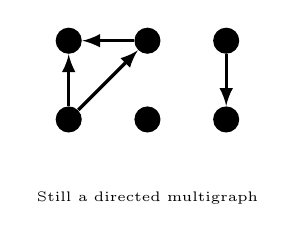
\begin{tikzpicture}
              \begin{scope}[every node/.style={fill=black, circle}]
                \node (a) at (0,0) {};
                \node (b) at (1,1) {};
                \node (c) at (0,1) {};
                \node (d) at (2,1) {};
                \node (e) at (2,0) {};
                \node (f) at (1,0) {};
              \end{scope}
              \begin{scope}[every edge/.style={draw=black, very thick, ->, >=latex}]
                \path (a) edge (b);
                \path (a) edge (c);
                \path (b) edge (c);
                \path (d) edge (e);
              \end{scope}
              \node at (1,-1) {\tiny Still a directed multigraph};
            \end{tikzpicture}
          \end{adjustbox}
        \end{center}
      \end{column}
    \end{columns}
    
  \end{frame}

  
\end{document}